\documentclass[a4paper,12pt]{report}

\usepackage{alltt, fancyvrb, url}
\usepackage{graphicx}
\usepackage[utf8]{inputenc}
\usepackage{float}
\usepackage{hyperref}

\usepackage[italian]{babel}

\usepackage[italian]{cleveref}

\title{Relazione \\``SMOL''}

\author{Ettore Farinelli \\ Marco Galeri \\ Giovanni Paradisi \\ Mounir Samite}
\date{\today}


\begin{document}

\maketitle

\tableofcontents


%------------------------------ANALISI------------------------------
\chapter{Analisi}

%REQUISITI
\section{Requisiti}
Il gruppo si pone come obiettivo quello di realizzare un videogioco 2D arcade con visuale dall’alto di nome "SMOL".
Per arcade si intende una struttura di gioco ripetitiva in cui l'obbiettivo è accumulare più punti possibile.
%

\subsubsection{Requisiti funzionali}
\begin{itemize}
    \item Il software dovrà essere in grado di gestire l'ambiente di gioco durante l'intera durata della partita elaborando le interazioni tra le diverse entità del gioco.
    \item L’obbiettivo del gioco è difendere i campi di ortaggi dalle talpe che invadono la mappa, schiacciandole con un martello. I campi subiranno danni anche in caso 
        il giocatore li attraversi.
    \item Con il progredire dello score la difficoltà di gioco aumenterà, diminuendo il tempo tra la creazione di talpe e modificando la probabilità 
        con cui si generano diversi tipi di talpa.
    \item Durante la partita sarà possibile effetuare diverse operazioni:
    \begin{itemize}
        \item Il giocatore potrà muovere il personaggio, attraverso i tasti direzionali, all’interno della mappa.
        \item Usando il mouse invece, controllerà la direzione del martello che attraverso una pressione prolungata potrà aumentare il raggio di azione.
    \end{itemize}
    \item Il gioco termina quando tutti gli ortaggi risultano distrutti.
\end{itemize}
\subsubsection{Requisiti non funzionali}
\begin{itemize}
    \item Si avrà la possibilità di cambiare l'aspetto grafico scegliendo tra quelli proposti nell'interfaccia del menù.
    \item Il programma sarà in grado di salvare il miglior punteggio in locale.
    \item Il gioco avrà una sezione in cui verrano visualizzate le istruzioni di gioco.
    \item Implementazione di una pagina di game over che permette di tornare al menù senza chiudere l'applicazione e 
        mantenendo lo stesso pacchetto grafico precedentemente utilizzato.
\end{itemize}
%ANALISI E MODELLO DEL DOMINIO
\section{Analisi e modello del dominio}
In SMOL il sofware dovrà essere in grado di controllare le interazioni tra diverse tipologie di entità. Tra le entità saranno presenti:
\begin{itemize}
    \item Ortaggi: queste entità fungeranno come vita del giocatore ed a contatto con altre entità perderanno vita
    \item Giocatore: questa entità sarà controllata attraverso la tastiera e permetterà di spostarsi all'interno della mappa.
    \item Martello: questa entità sarà controllata attraverso il mouse che con una pressione prolungata permetterà di aumentare il proprio raggio di azione, mentre al rilascio se si troverà a contatto con le talpe gli toglierà vita
    \item Talpe: questa entità fungerà da nemico principale del giocatore, spostandosi attraverso la mappa cercherà di mangiare gli ortaggi presenti ed in caso entri in contatto col giocatore gli bloccherà temporaneamente i movimenti.
    \item Muri: impediranno al giocatore di uscire dai confini della mappa di gioco
\end{itemize}
Il sofware sarà responsabile anche della generazione iniziale degli ortaggi e la generazione delle talpe durante il resto della partita attraverso un sistema che incrementerà il numero di talpe generate nel tempo in base al punteggio corrente del giocatore.
Gli elementi costitutivi del dominio sono sintetizzati in \Cref{img:analysisScheme}.
Per rientrare nel monte ore richiesto non è stato possibile implementare una modalità di multiplayer locale, che sarà possibilmente implementata in futuro.

\begin{figure}[H]
\centering{}
%\includegraphics{img/analysisScheme}
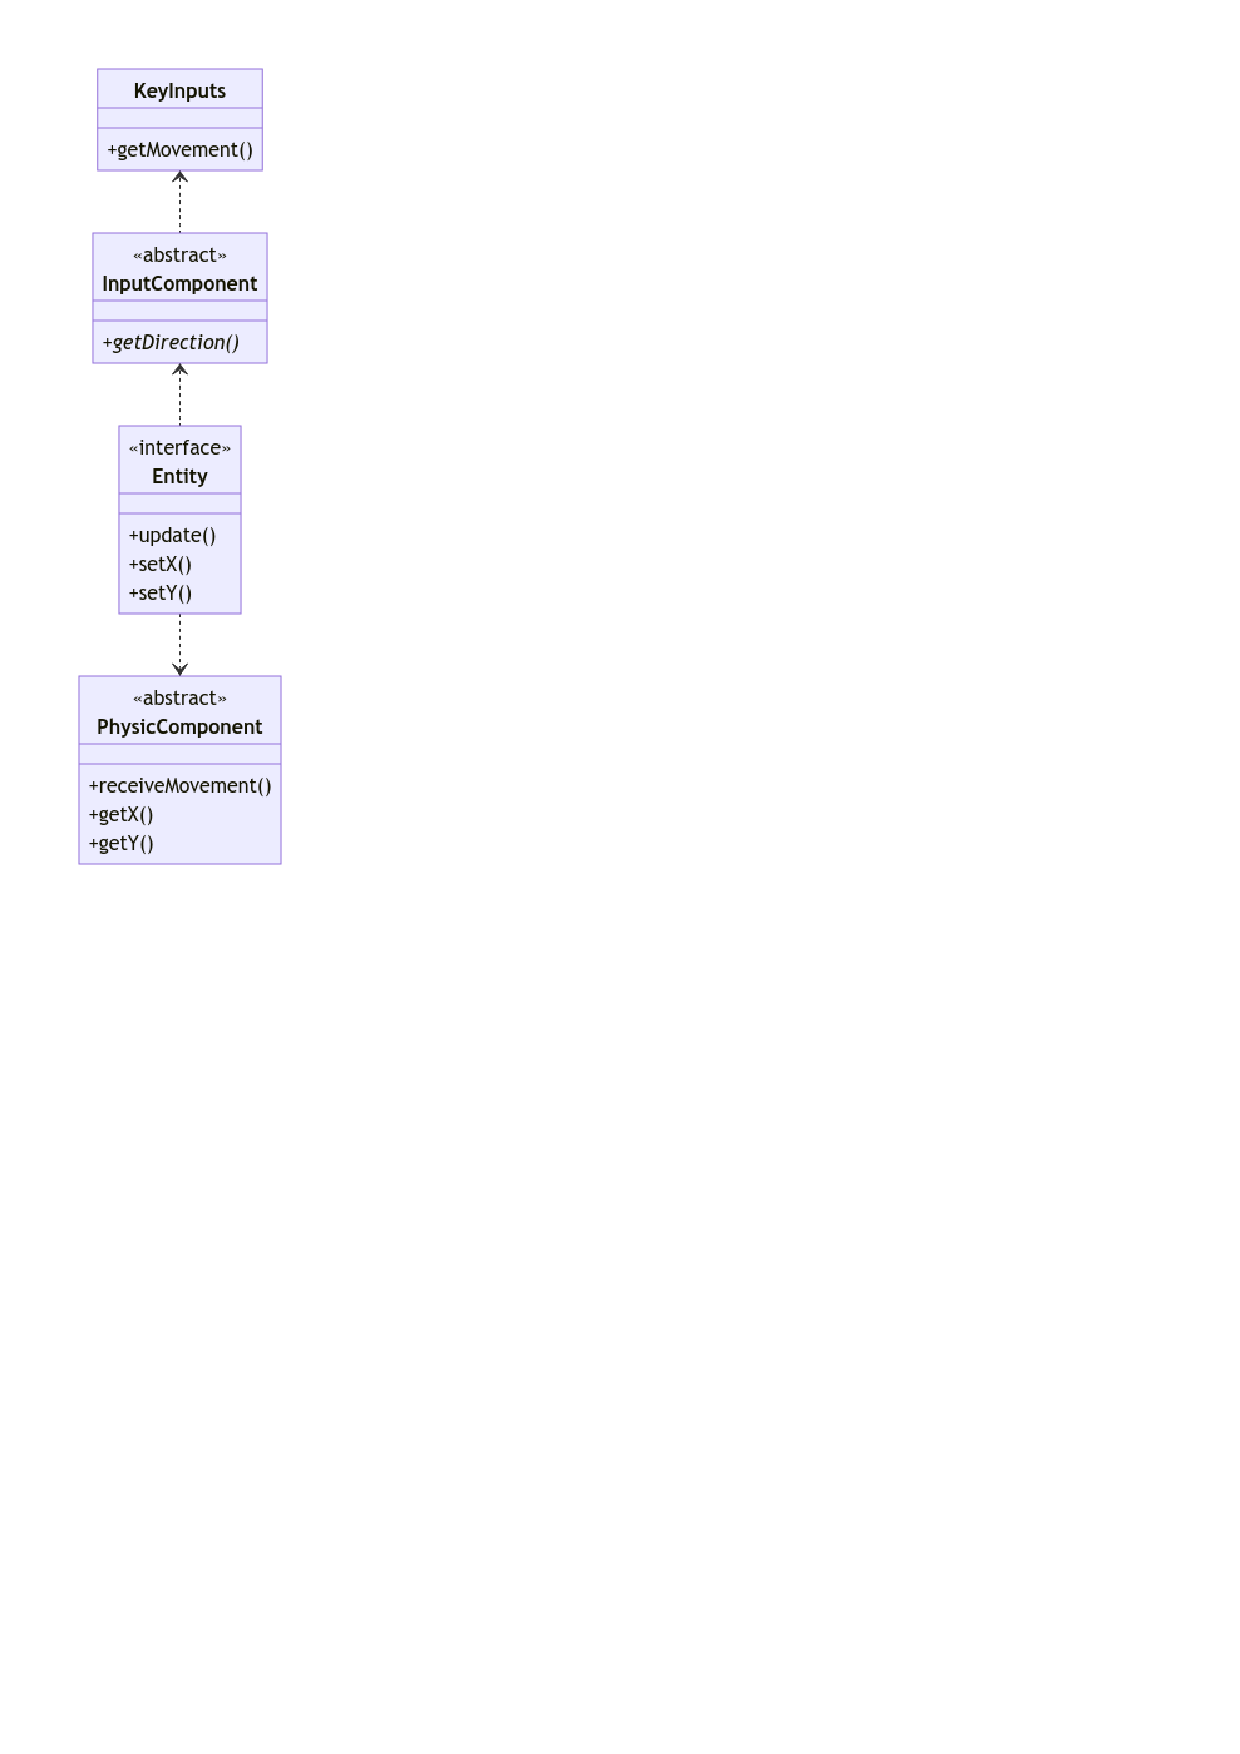
\includegraphics{img/PlayerMovementUML.pdf}
\caption{Schema UML dell'analisi del problema, con rappresentate le entità principali ed i rapporti fra loro}
\label{img:analysisScheme}
\end{figure}

%------------------------------DESIGN------------------------------
\chapter{Design}

%ARCHITETTURA
\section{Architettura}

L'architettura di GLaDOS segue il pattern architetturale MVC.
%
Più nello specifico, a livello architetturale, si è scelto di utilizzare MVC in forma ``ECB'', ossia ``entity-control-boundary''\footnote{
Si fa presente che il pattern ECB effettivamente esiste in letteratura come ``istanza'' di MVC, e chi volesse può utilizzarlo come reificazione di MVC.
}.
%
GLaDOS implementa l'interfaccia AI, ed è il controller del sistema.
Essendo una intelligenza artificiale, è una classe attiva.
%
GLaDOS accetta la registrazione di Input ed Output, che fanno parte della ``view'' di MVC, e sono il ``boundary'' di ECB.
Gli Input rappresentano delle nuove informazioni che vengono fornite all'IA, ad esempio delle modifiche nel valore di un sensore, oppure un comando da parte dell'operatore.
Questi input infatti forniscono eventi.
Ottenere un evento è un'operazione bloccante: chi la esegue resta in attesa di un effettivo evento.
Di fatto, quindi, GLaDOS si configura come entità \textit{reattiva}.
Ogni volta che c'è un cambio alla situazione del soggetto, GLaDOS notifica i suoi Output,
informandoli su quale sia la situazione corrente.
%
Conseguentemente, GLaDOS è un ``observable'' per Output.

\begin{figure}[h]
\centering{}
%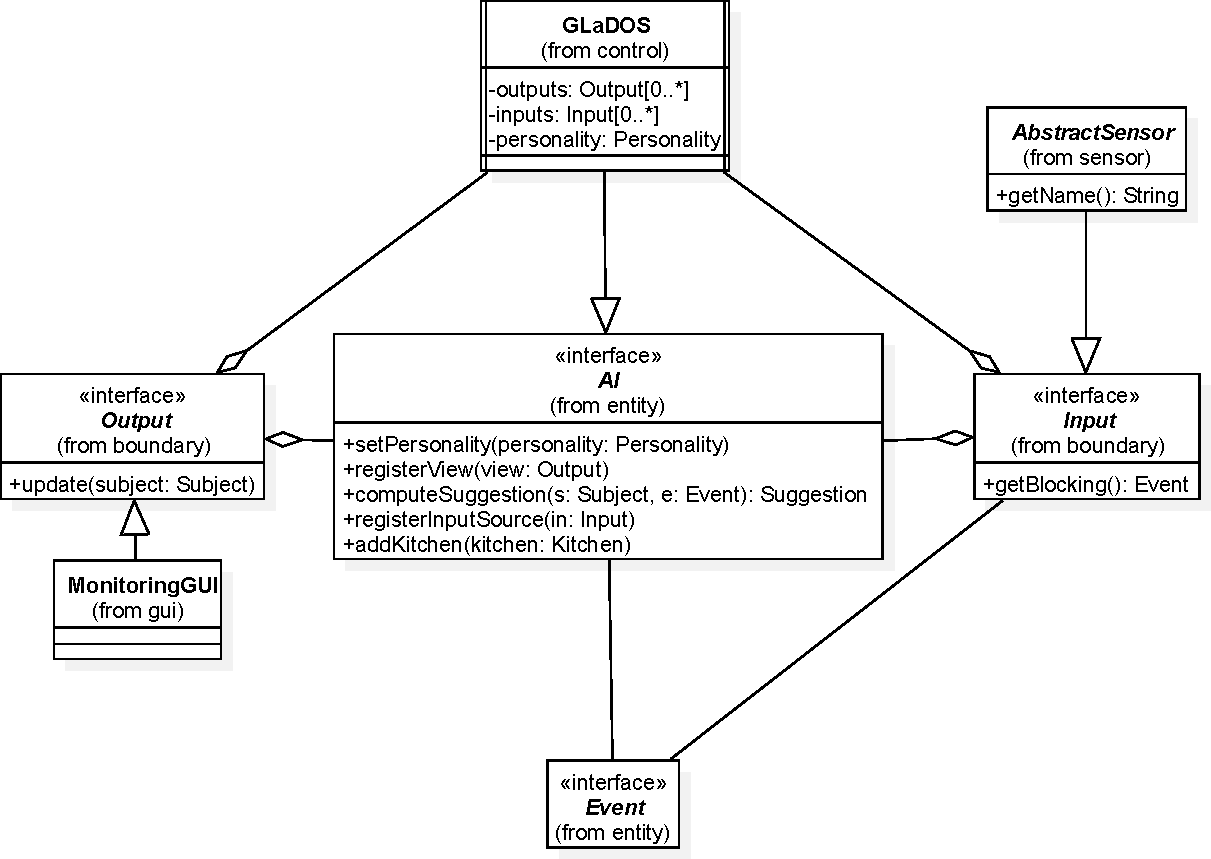
\includegraphics[width=\textwidth]{img/arch}
\caption{Schema UML architetturale di GLaDOS. L'interfaccia \texttt{GLaDOS} è il controller del sistema, mentre \texttt{Input} ed \texttt{Output} sono le interfacce che mappano la view (o, più correttamente in questo specifico esempio, il boundary). Un'eventuale interfaccia grafica interattiva dovrà implementarle entrambe.}
\label{img:goodarch}
\end{figure}

Con questa architettura, possono essere aggiunti un numero arbitrario di input ed output
all'intelligenza artificiale.
%
Ovviamente, mentre l'aggiunta di output è semplice e non richiede alcuna modifica all'IA, la
presenza di nuovi tipi di evento richiede invece in potenza aggiunte o rifiniture a GLaDOS.
%
Questo è dovuto al fatto che nuovi Input rappresentano di fatto nuovi elementi della business
logic, la cui alterazione od espansione inevitabilmente impatta il controller del progetto.

In \Cref{img:goodarch} è esemplificato il diagramma UML architetturale.

%DESIGN DETTAGLIATO%DESIGN DETTAGLIATO
\section{Design dettagliato}

\subsection*{Ettore Farinelli}
roba di Ettore
\subsection*{Marco Galeri}

\subsubsection{Gestione delle Entità}

\begin{figure}[H]
\centering{}
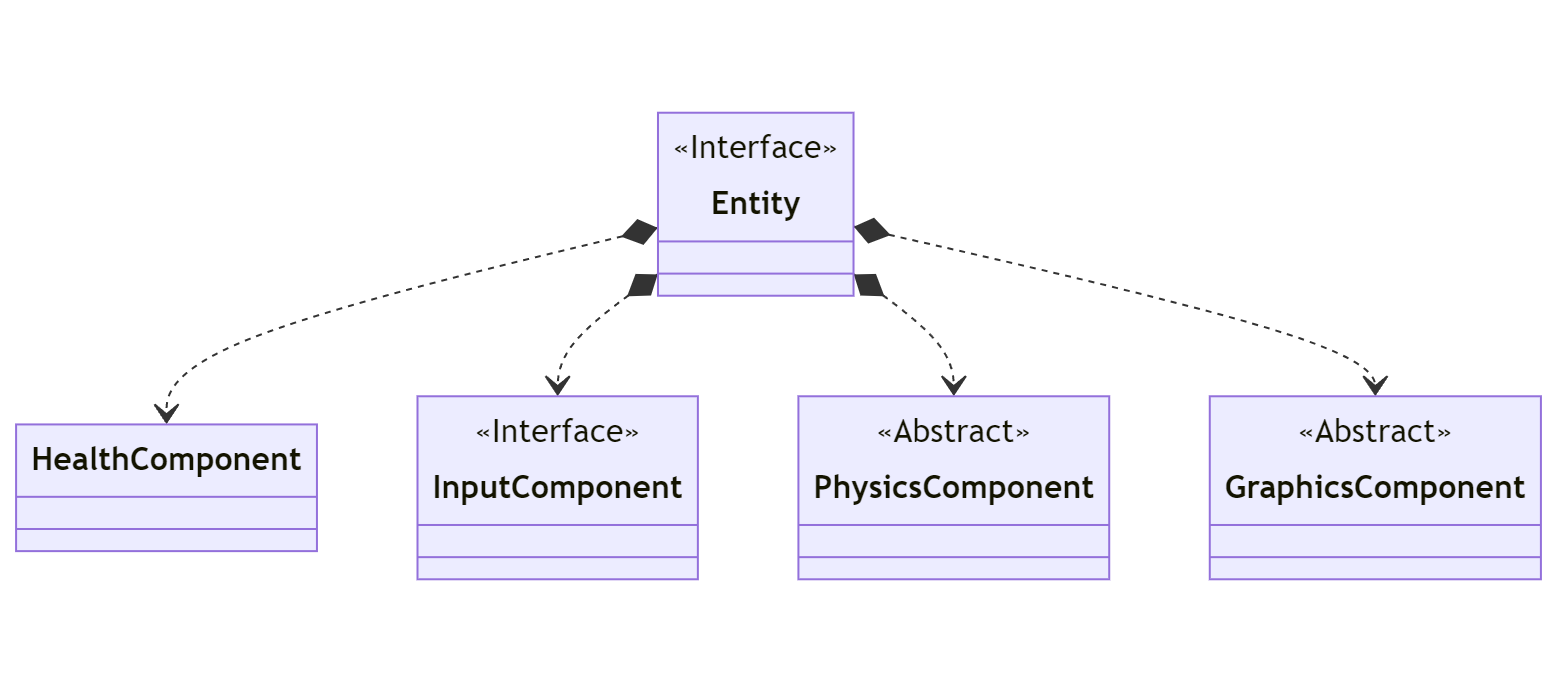
\includegraphics{img/EntityUML.pdf}
\caption{Rappresentazione UML di una entità e i suoi componenti}
\end{figure}

\paragraph{Problema}
    L'interfaccia \textsc{Entity} deve implementare numerosi comportamenti diversi, l'uso dell'ereditarietà porterebbe alla creazione di molteplici sottoclassi ed a possibili problemi di eredità multipla aumentando la complessità del codice. Inoltre la classe \textsc{Entity} incapsula diversi aspetti del gioco violando il \textit{Single Responsability Principle}.

\paragraph{Soluzione}
    Adottando l'\textit{Entity Component System}, ampiamente usato nell'ambito di Game Development, si ha una scissione dei vari aspetti di gioco in \textsc{components}. L'unione dei \textsc{components} quindi definisce il comportamento finale di ogni Entità. Con questo design che favorisce la composizione al posto dell'ereditarietà si ha un aumento di flessibilità del codice che viene suddiviso in classi più corte e meno complicate. Inoltre i componenti sono altamente riusabili rendendo plausibile la creazione di diverse tipologie di entità e lasciando libera la possibilità di aggiunte future.

\subsubsection{Creazione delle Entità}

\begin{figure}[H]
\centering{}
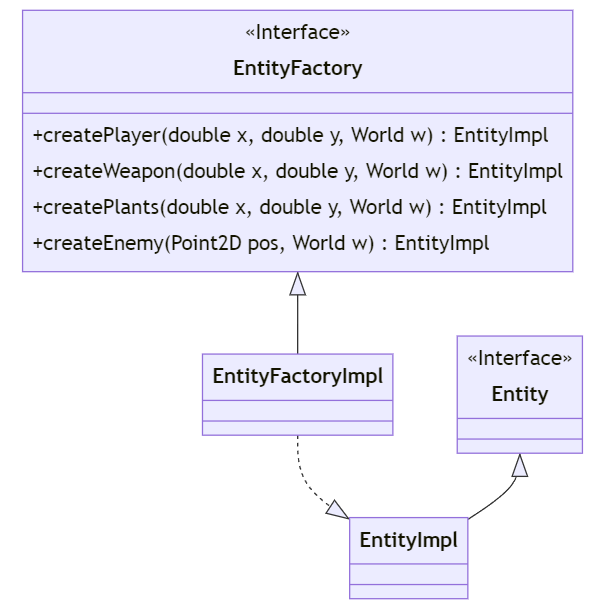
\includegraphics{EntityFactoryUML.pdf}
\caption{Rappresentazione UML della creazione di una entità attraverso l'utilizzo del Factory method}
\end{figure}

\paragraph{Problema}
    Date le molteplici tipologie di componenti che una Entità può avere, la creazione di un'Entità direttamente all'interno del mondo è possibile ma poco flessibile e funzionale. 
    
\paragraph{Soluzione}
    Impiegando il \textit{Factory design pattern},  la creazione dell'entità viene esternalizzata in una classe. Con questa classe, \textsc{EntityFactory}, si possono creare dei set di componenti predefiniti da usare per istanziare ogni tipo di entità. Attraverso questo metodo si diminuisce notevolmente la duplicazione di codice, inoltre si rimuove la responsabilità di creazione delle entità dalla classe chiamante. 
    
\subsection*{Giovanni Paradisi}
roba di Giovanni
\subsection*{Mounir Samite}
roba di Mounir


%------------------------------SVILUPPO------------------------------
\chapter{Sviluppo}

%TESTING
\section{Testing automatizzato}

%METODOLOGIA_DI_LAVORO
\section{Metodologia di lavoro}
un po di roba sul DVCS

\subsection*{Ettore Farinelli}
roba di Ettore
\subsection*{Marco Galeri}
roba di Marco
\subsection*{Giovanni Paradisi}
roba di Giovanni
\subsection*{Mounir Samite}
Mi sono occupato di:
\begin{itemize}
    \item Progettazione dell'utilizzo delle finestre con \emph{Window} e \emph{WindowState} con cui verranno renderizzate tutti i tipi di finestre come Menu, Gioco e Game Over (\textbf{package it.unibo.smol.view});
    \item Implementazione del Menu di gioco nella classe \emph{MenuState} (\textbf{package it.unibo.smol.view});
    \item Implementazione del GameOver (fine gioco) nella classe \emph{GameOverWinState} (\textbf{package it.unibo.smol.view});
    \item Progettazione del Mondo di gioco ovvero del contenitore di tutte le entità, degli input e dello score andando a gestire alcune loro funzionalità in \emph{WorldImpl} (\textbf{package it.unibo.smol.model});
    \item Progettazione della barra della vita del player in \emph{HealthBarTankImpl} (\textbf{package it.unibo.smol.view}).
\end{itemize}
Ho inoltre contribuito a:
\begin{itemize}
    \item \emph{PlayerInputComponent} (\textbf{package it.unibo.smol.controller});
    \item \emph{WeaponInputComponent} (\textbf{package it.unibo.smol.controller});
    \item \emph{GameViewState} andando a gestire la barra della vita anche li (\textbf{package it.unibo.smol.view});
    \item \emph{GameEngine} aggiungendo le skins (che in questo caso sono intese come diversi tipi di grafica) al gioco: vettoriale e pixelata per ora (\textbf{package it.unibo.smol.core}) 
\end{itemize}

%NOTE_DI_SVILUPPO
\section{Note di sviluppo}
Siamo partiti inizialmente con un'attenta analisi del dominio del gioco e di cosa potesse essere aggiunto, cercando di rendere il gioco adeguatamente estendibile.
Dunque è stato fatto un UML generale per avere in mente il funzionamento del gioco e sono state definite tutte le principali interfacce.
Invece per quanto riguarda il workflow è stata adottata la metodologia di DVCS semplice, spiegata a lezione, con pull e push.
\subsection*{Ettore Farinelli}
roba di Ettore
\subsection*{Marco Galeri}
roba di Marco
\subsection*{Giovanni Paradisi}
roba di Giovanni
\subsection*{Mounir Samite}
\subsubsection*{Utilizzo di Stream per gestione delle entità}
\begin{itemize}
    \item Prendere le talpe dalla lista di entità: \url{https://github.com/TheDarkRuler/OOP22-SMOL/blob/dac2df26a7ed60c955c6ea339cb908958a450955/src/main/java/it/unibo/smol/model/impl/WorldImpl.java#L49-L55}
    \item Prendere le piante dalla lista di entità: \url{https://github.com/TheDarkRuler/OOP22-SMOL/blob/dac2df26a7ed60c955c6ea339cb908958a450955/src/main/java/it/unibo/smol/model/impl/WorldImpl.java#L63-L69}
    \item Rileva il player dalla lista di entità: \url{https://github.com/TheDarkRuler/OOP22-SMOL/blob/dac2df26a7ed60c955c6ea339cb908958a450955/src/main/java/it/unibo/smol/model/impl/WorldImpl.java#L56-L62}
\end{itemize}



%------------------------------COMMENTI_FINALI------------------------------
\chapter{Commenti finali}

un po de roba

%AUTOVALUTAZIONE_E_LAVORI_FUTURI
\section{Autovalutazione e lavori futuri}
\subsection*{Ettore Farinelli}
roba di Ettore
\subsection*{Marco Galeri}
roba di Marco
\subsection*{Giovanni Paradisi}
roba di Giovanni
\subsection*{Mounir Samite}
roba di Mounir

%DIFFICOLTA(OPZIONALE)
\section{Difficoltà incontrate e commenti per i docenti}

\textbf{opzionale}



\appendix

%------------------------------GUIDA------------------------------

\chapter{Guida utente}



\bibliographystyle{alpha}
\bibliography{report}

\end{document}
